\documentclass[twocolumn]{article}

\usepackage{amsmath}
\usepackage{caption}
\usepackage{graphicx}
\usepackage{float}
\usepackage{subcaption}
\usepackage{gensymb}

% Make table names in captions boldfaced
\captionsetup[table]{labelfont=bf}
\captionsetup[figure]{labelfont=bf}

%opening
\title{Laboratory Observations of the Zeeman Effect}
\author{Jack Nelson,\\
	Physics Department,\\
	Occidental College, Los Angeles, CA}
\date{November 2016}

\begin{document}

\maketitle

\begin{abstract}
	
\end{abstract}

\section{Introduction} \label{sec:Intro}
	\subsection{Historical Background}

	\subsection{Theoretical Overview} \label{sec:Theory}
		The splitting of the spectra of mercury into hyperfine lines when an external magnetic field is applied is the result of the mercury atom's magnetic-dipole interaction with the external magnetic field.
		 
		In its ground state, the mercury atom has 80 electrons in which the n = 1, 2, 3, 4, and 5 shells are filled, leaving two 6s valence electrons.
		The spectral emissions of mercury come from the transitions of these two valence electrons between different quantum states.
		Figure \ref{fig:MercuryEnergyLevelsDiagram} shows the different possible transitions of the mercury atom.
		Our observations will be limited to the $7^3S_1 \rightarrow 6^3P_2$ transition which yields the 546.1 nm green spectral line.
		
		When no external magnetic field is present, hyperfine structure in atomic spectra can be observed due to the spin-angular momentum coupling of electrons. 
		See pp. 47 of \cite{melissinos_experiments_1966} for a more detailed discussion.
		In the presence of an external magnetic field, the interaction of the total angular momentum of the electrons with the magnetic field also splits the spectral lines into finer lines of slightly different wavelength.
		Figure \ref{fig:SpectralSplitting} shows how a single transition from the $l=2$ to $l=1$ states results in hyperfine structure in the presence of a magnetic field.
		
		\begin{figure}
			\centering
			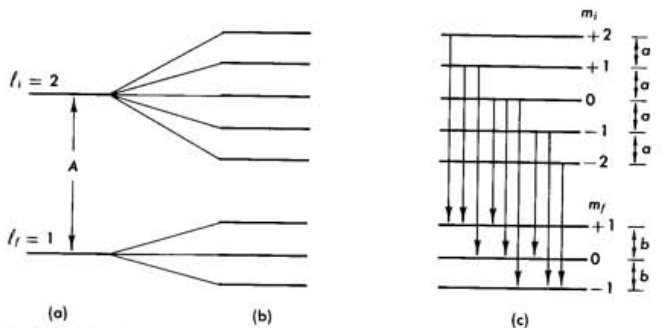
\includegraphics[width=1.0\linewidth]{Images/SpectralSplitting}
			\caption{A single spectral line caused by an atomic energy transition will be split into multiple ``hyperfine" lines due to the interaction of the total angular momentum of the valence electrons with an external magnetic field. (a) shows the transition in the absence of an external magnetic field. The transition between the $l=2$ and the $l=1$ states ($d\rightarrow p$) produces a single spectral line. (b) shows how these formerly single energy-levels are split into multiple states in the presence of an external magnetic field. (c) shows the possible transitions between the new states, each of which produces a different spectral line with slightly different wavelength.}
			\label{fig:SpectralSplitting}
		\end{figure}
		
		The following discussion is a summary of that in chapter 2 of \cite{melissinos_experiments_1966} on the Zeeman Effect.
		For a more detailed discussion of the derivation and consequences, consult that reference.
		
		Hyperfine splitting in the presence of a magnetic field is due to the interactions of the valence electrons with the magnetic field.
		These interactions result in an added energy $\Delta E$ per electron given by
		\begin{equation}
			\Delta E = m\mu_0H
		\end{equation}
		where $m$ is the mass of the electron, $\mu_0$ is the Bohr Magneton, fundamental magnetic moment of the electron, and $H$ is the applied magnetic field.
		
		The Bohr Magneton arises from modeling the electron classically as a current loop with current density
		\begin{equation}
			\mathbf{J(x)} = -e\mathbf{v} \delta\left(\mathbf{x} - \mathbf{r}\right)
		\end{equation}
		Where $\mathbf{r}$ is the orbit equation and $\mathbf{x}$ is the electron position.
		
		This current density results in a magnetic dipole moment given by
		\begin{equation}
			\mathbf{u} = \frac{1}{2c}\int \mathbf{x} \times \mathbf{J(x)} d^3x = -\frac{1}{2c}e\left(\mathbf{r \times v}\right)
		\end{equation}
		The angular momentum of the orbit is given by
		\begin{equation}
			\mathbf{L} = \mathbf{r \times p} = m_e\left(\mathbf{r \times v}\right)
		\end{equation}
		
		The quantized angular momentum of the electron is given by 
		\begin{equation}
			\mathbf{L} = \frac{lh}{2\pi}
		\end{equation}
		
		The total angular momentum $j$ of mercury is dependent on both the orbital angular momentum of the valence electrons given by the quantum number $l$, and the spin angular momentum quantum number $s$.
		In Russell-Saunders or LS coupling, the total angular momentum is given by the sum of the orbital angular momentum and the spin angular momentum:
		
		\begin{equation}
			j = l + s
			\label{eq:TotalAngularP}
		\end{equation}
		Figure \ref{fig:TotalAngularMomentumDiagram} shows how these two quantities (vectors, actually) combine to form total angular momentum.
		
		\begin{figure}
			\centering
			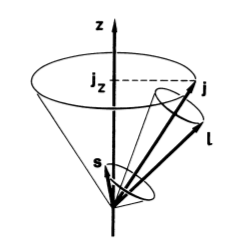
\includegraphics[width=0.90\linewidth]{Images/TotalAngularMomentumDiagram}
			\caption{Electron spin angular momentum $\mathbf{s}$ and orbital angular momentum $\mathbf{l}$ sum to create total angular momentum $\mathbf{j}$.}
			\label{fig:TotalAngularMomentumDiagram}
		\end{figure}

		
		Selection rules place restrictions on how the quantum numbers may change when a valence electron undergoes a transitions.
		These selection rules are:
		\begin{enumerate}
			\item $\Delta s = 0$
			\item $\Delta l = 0, \pm1$
			\item $\Delta J = 0, \pm1$, but not $\Delta J = 0 \rightarrow \Delta J = 0$
			\item $\Delta M_j = 0, \pm1$, but not $M_j=0\rightarrow M_j=0$ if $\Delta J = 0$
		\end{enumerate}
		
		Figure \ref{fig:SpectralSplitting} shows that spectral splitting is dependent on the magnetic quantum number $m$ which specifies the projection of the orbital angular momentum along the z-axis of the atom.
		$m$ can take on $2l+1$ the values ranging from $l$ to $-l$.
		
		The polarization of the emitted light during the transition is also entirely determined by $\Delta m_j$.
		For $\Delta m_j = 0$, the emitted photons are polarized linearly and parallel to the field lines of the applied magnetic field $\mathbf{B}$.
		For $\Delta m_j=\pm1$, emitted photons are circularly polarized along the direction of $\mathbf{B}$ and appear linearly polarized perpendicular to $\mathbf{B}$ when viewed side-on to $\mathbf{B}$.
		\begin{figure}
			\centering
			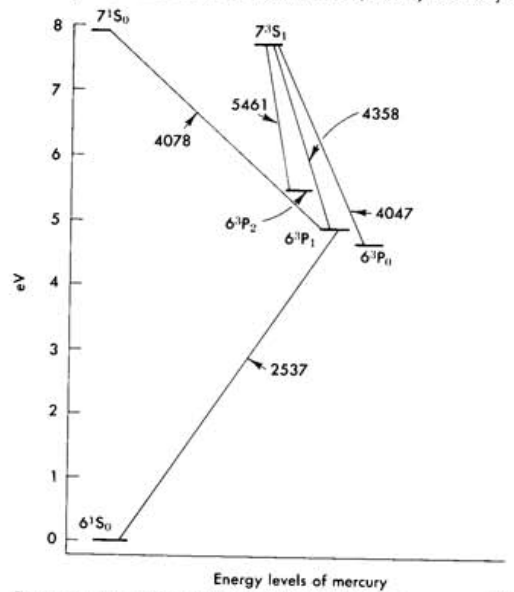
\includegraphics[width=0.5\textwidth]{Images/MercuryEnergyLevelsDiagram.png}
			\caption{Energy level transitions of mercury between quantum states. For the purposes of our observations, we are interested in the $7^3S_1 \rightarrow 6^3P_2$ transition which produces 546.1 nm light. Figure 7.39 of \cite{melissinos_experiments_1966}}
			\label{fig:MercuryEnergyLevelsDiagram}
		\end{figure}
		
		The energy difference between the hyperfine spectra is caused by the differing values of $\Delta m$ and determined by measuring the relative differences in wavelength between the fine spectra.
		From the basic Planck relation we have
		\begin{equation}
			E = h\nu = \frac{hc}{\lambda}
		\end{equation}
		where $h$ is the Planck constant, $\nu$ is wave frequency, and $\lambda$ is wavelength.
		
		The relative energy difference of two wavelengths is then given by
		\begin{equation}
			\Delta E = -\left(\frac{hc}{\lambda^2}\right) \Delta \lambda
		\end{equation}
	

		
\section{Methods and Procedures}
	The Pasco Scientific Model SE-9654 Zeeman Effect Experiment was used to make all observations.
	The experiment consisted of two large solenoids oriented along the same axis with an air gap between them in which a mercury lamp was placed.
	An optical rail was used to align a polarizing filter, a collimating lens, an interference filter, a Fabry-Perot interferometer, and a CMOS camera.
	The basic experimental technique consisted of imaging the interference pattern of the 546.1 nm mercury spectral line through the polarizer and Fabry-Perot interferometer.
	Figure 
	
	\begin{figure*}
		\centering
		\begin{subfigure}{0.5\textwidth}
			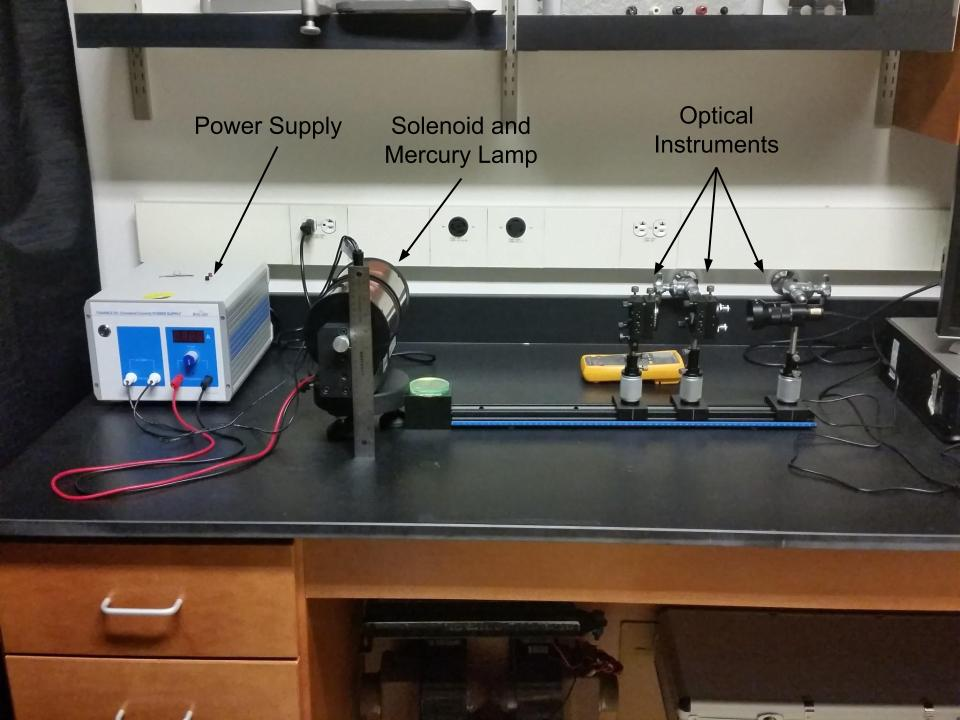
\includegraphics[width = 0.8\textwidth]{Images/ExperimentOverview.jpg}
			\caption{}
			\label{subfig:Overview}
			
		\end{subfigure}%
		\begin{subfigure}{0.5\textwidth}
				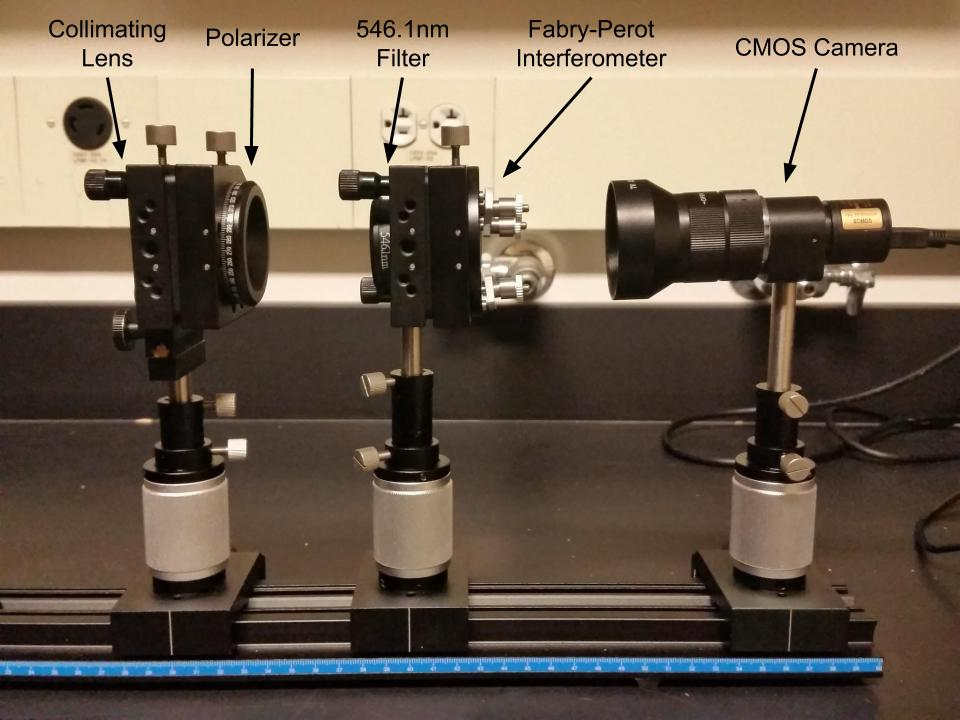
\includegraphics[width = 0.8\textwidth]{Images/OpticsRail.jpg}
				\caption{}
				\label{subfig:OpticsRail}
				
		\end{subfigure}%
		\caption{\textbf{Overview of the Experiment configuration. Figure \ref{subfig:Overview} shows the entire apparatus with the variable power supply for the solenoid and mercury lamp, the solenoid, the mercury lamp (hidden by the solenoid), the optical track, and the optical instruments. Figure \ref{subfig:OpticsRail} shows the optical instruments in detail.}}
		\label{fig:ContextView}
	\end{figure*}
	
	\begin{figure*}
		\centering
		\begin{subfigure}{0.5\textwidth}
			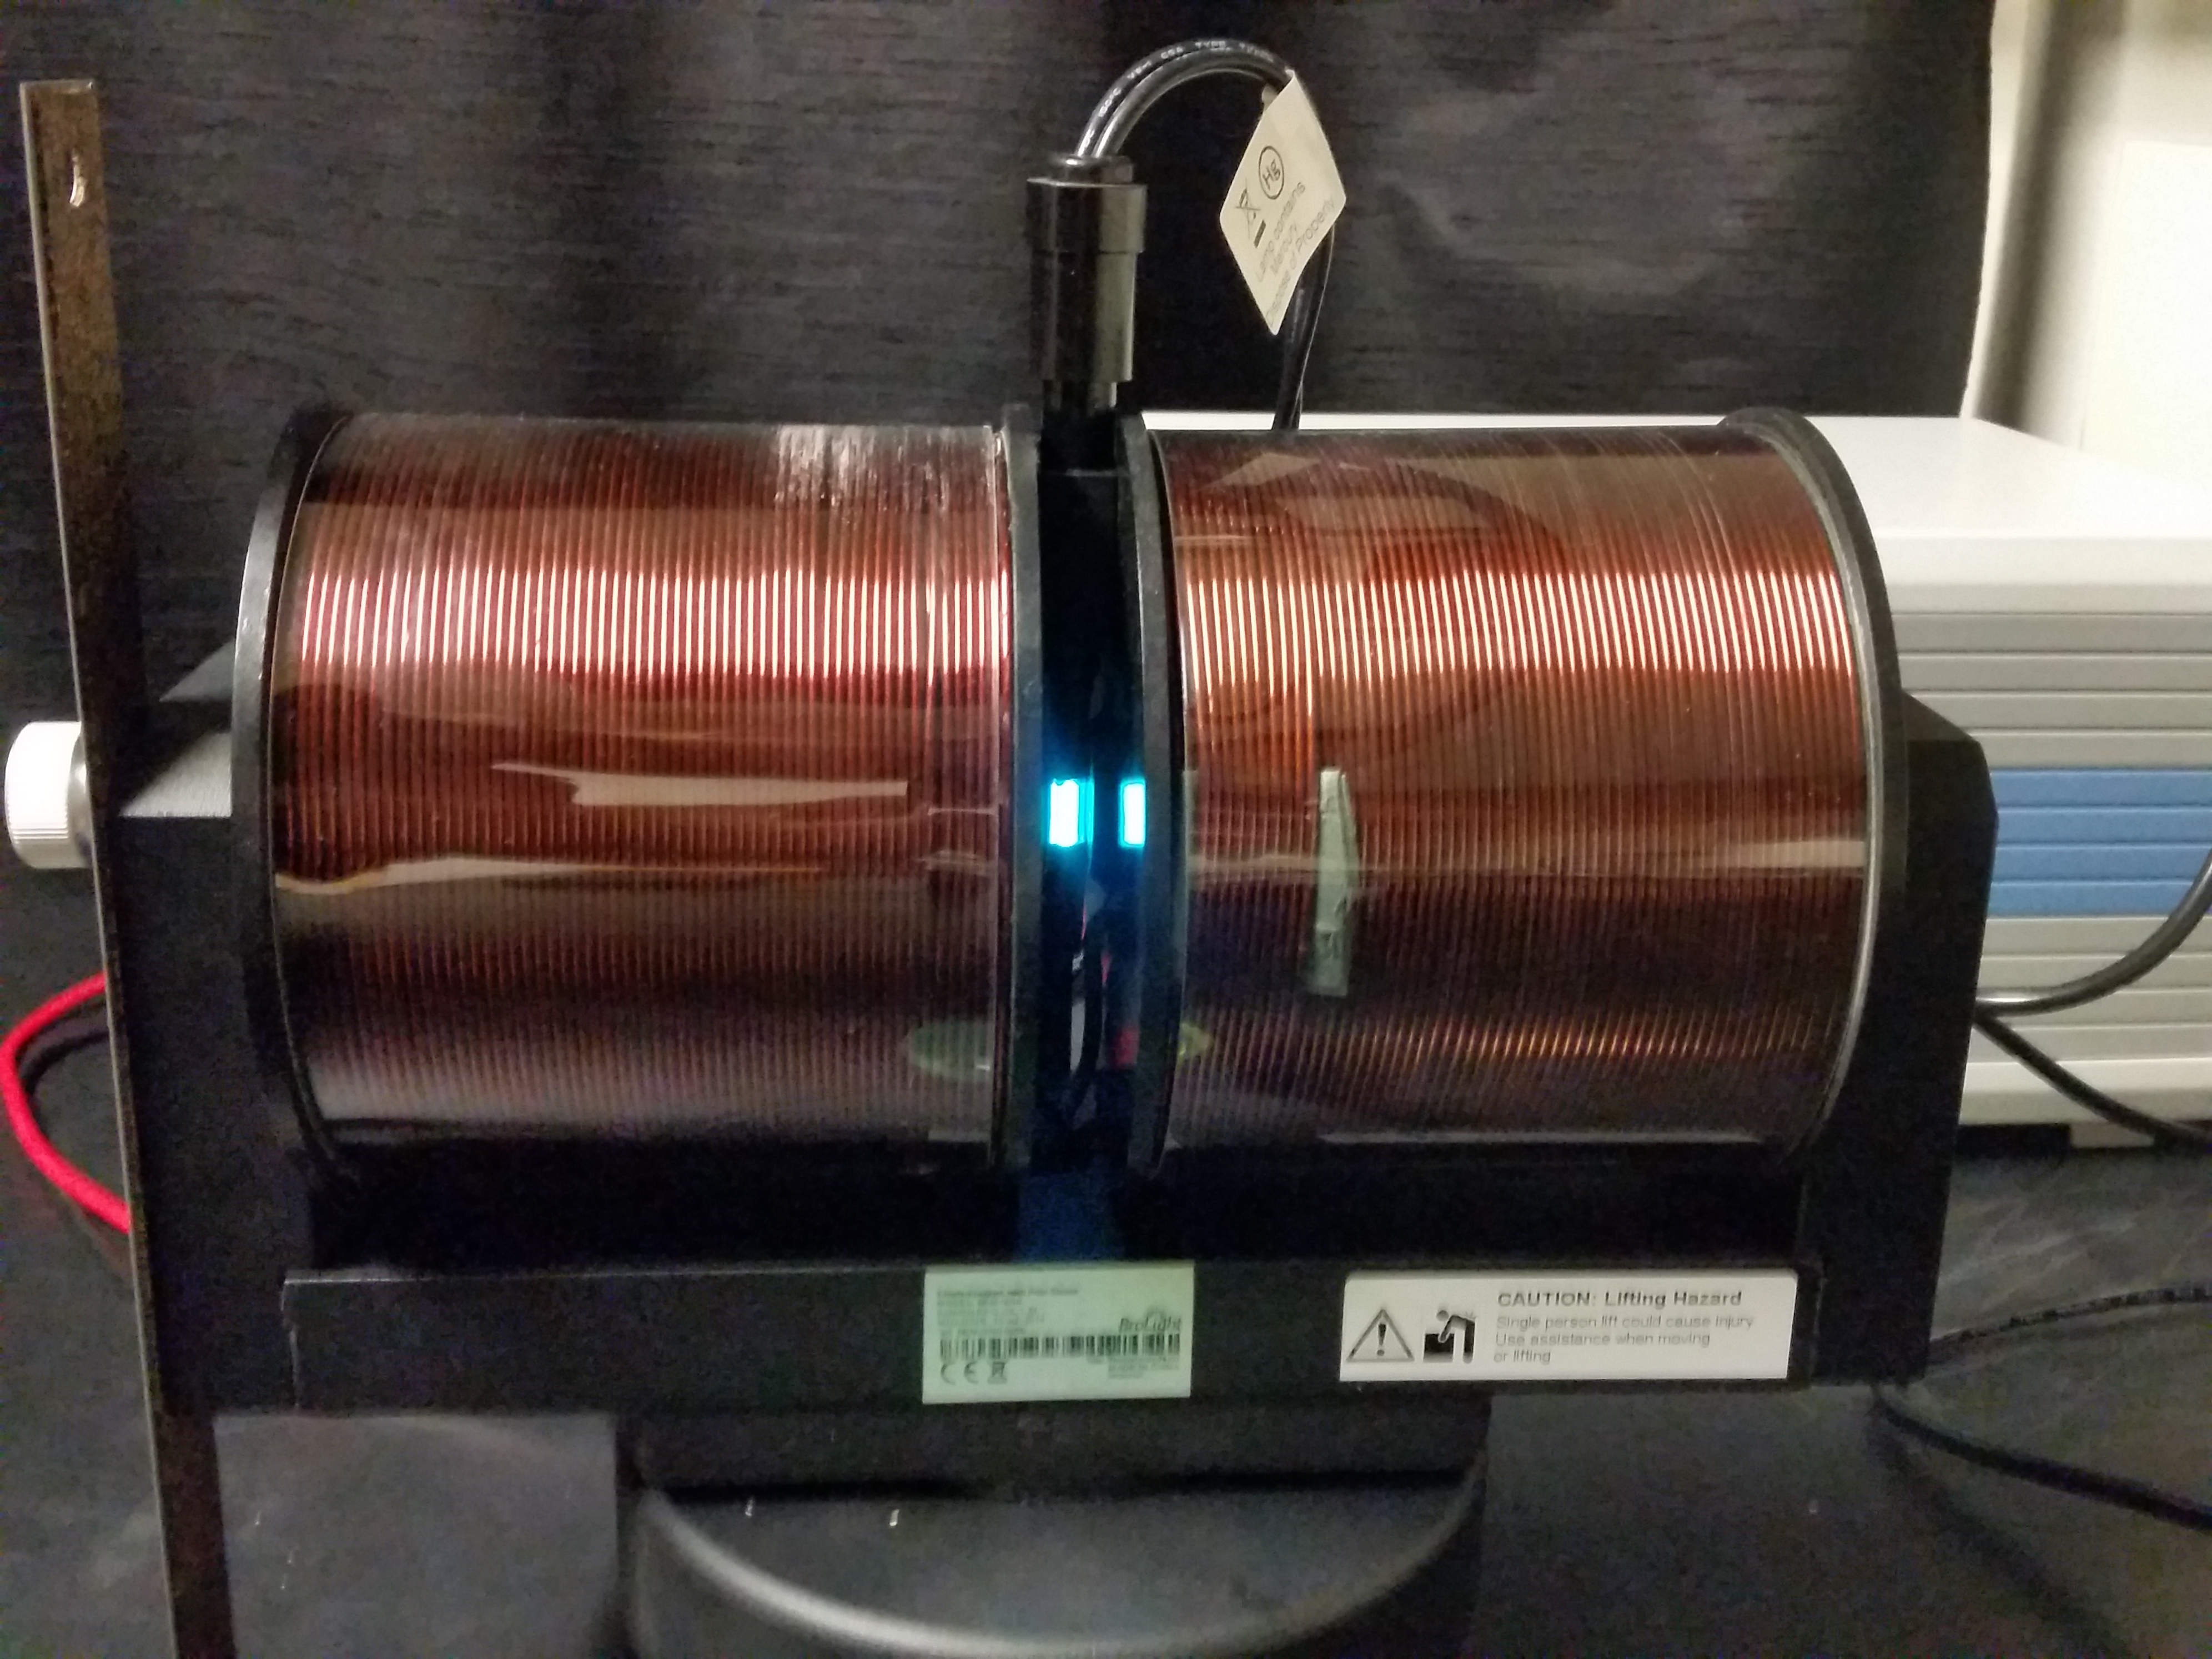
\includegraphics[width = 0.8\textwidth]{Images/PerpendicularView.jpg}
			\caption{}
			\label{subfig:PerpView}
		\end{subfigure}%
		\begin{subfigure}{0.5\textwidth}
			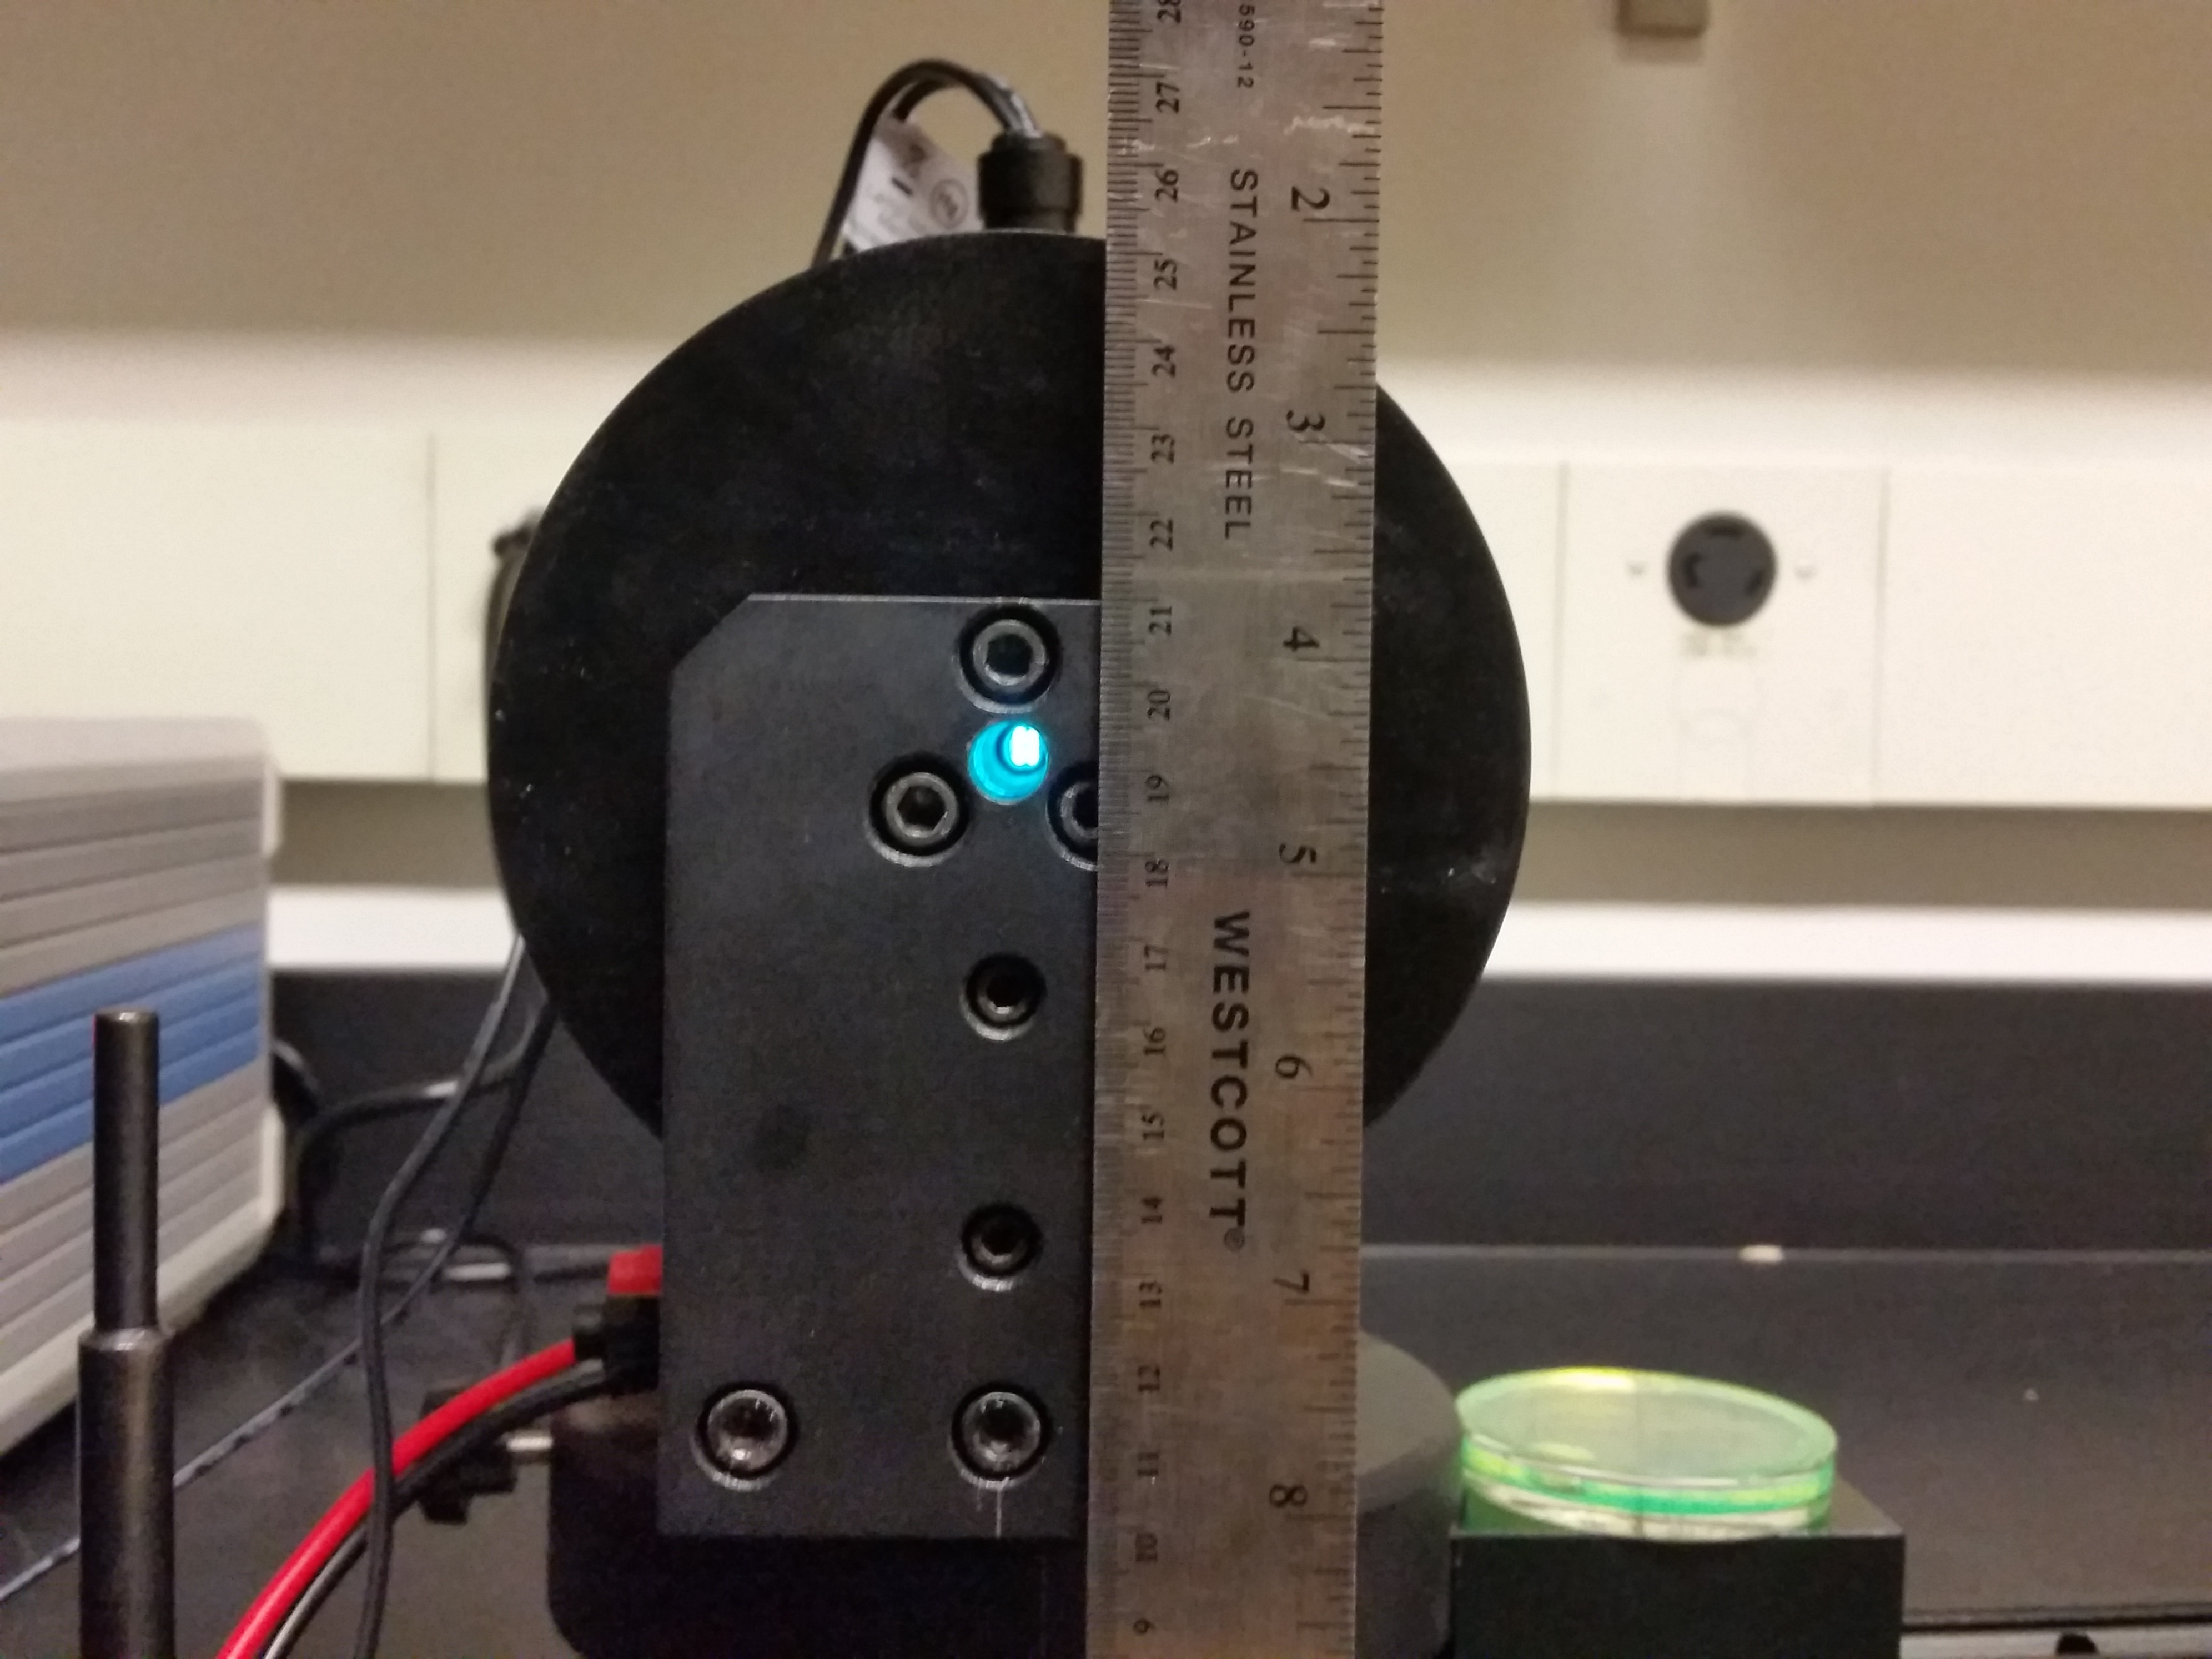
\includegraphics[width = 0.8\textwidth]{Images/AxialView.jpg}
			\caption{}
			\label{subfig:AxialView}
		\end{subfigure}%
		\caption{\textbf{Detail view of the solenoid with the mercury lamp source. Figure \ref{subfig:PerpView} shows the configuration with the magnetic field lines perpendicular to the light source. Figure \ref{subfig:AxialView} shows the axial field configuration looking down the sight-hole of the solenoid to the mercury lamp.}}
		\label{fig:SolenoidDetail}
	\end{figure*}
	
	
	
	To study the Zeeman effect, observations of a mercury lamp were made first with no magnetic field and $90\deg$ polarization, then with an approximately $1T$ magnetic field.
	Observations with a magnetic field included:
	\begin{itemize}
		\item $90\deg$ (field-perpendicular) polarization
		\item $0\deg$ (field-parallel) polarization 
		\item No polarization
		\item Axial B-field at polarization varying from $90\deg$ to $0\deg$
	\end{itemize}
	
	Figure \ref{fig:FieldConfig} shows the perpendicular and axial configurations of the magnetic field used for the observations.
	
	The observations and results of each of these field configurations will be presented and discussed in Section \ref{sec:DataAndResults}.
	
	 
	
	
	\begin{figure*}
		\centering
		\begin{subfigure}{0.55\textwidth}
			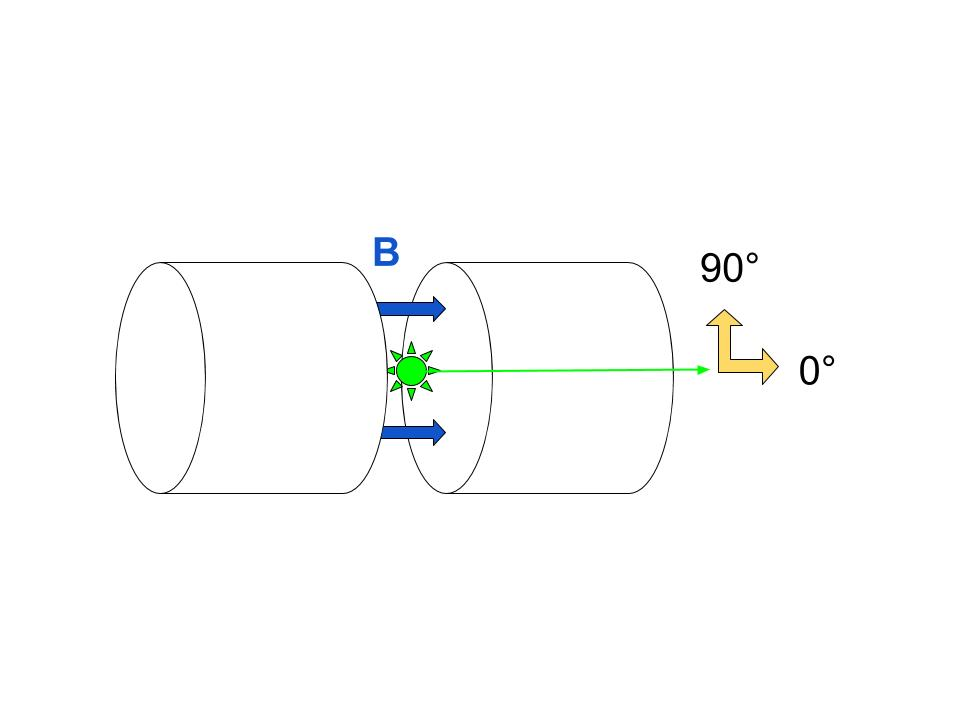
\includegraphics[width = 1.0\textwidth]{Images/FieldConfigA.jpg}
			\caption{\textbf{Perpendicular field configuration.}}
			\label{subfig:PerpFieldConfig}
		\end{subfigure}%
		\begin{subfigure}{0.55\textwidth}
			\centering
			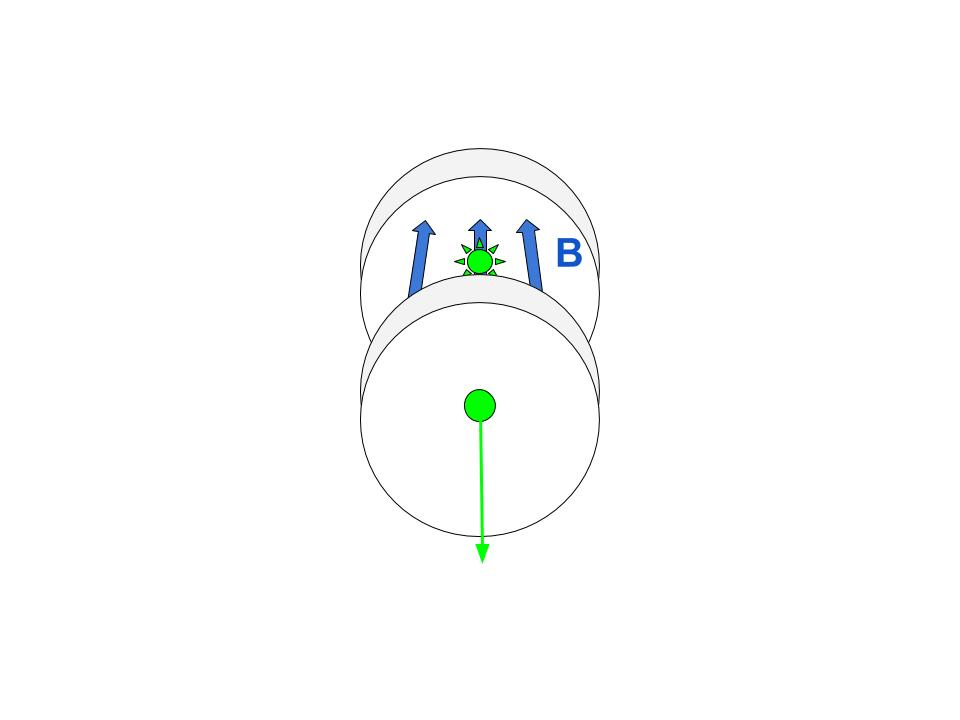
\includegraphics[width=1.0\textwidth]{Images/FieldConfigB.jpg}
			\caption{\textbf{Axial field configuration.}}
			\label{subfig:AxialFieldConfig}
		\end{subfigure}%
		\caption{\textbf{The two magnetic field configurations observed. In (\ref{subfig:PerpFieldConfig}), the magnetic field is oriented perpendicularly to the path of the observed light from the mercury lamp. $\mathbf{90\degree}$ polarization is defined to be perpendicular to the field lines, while $\mathbf{0\degree}$ polarization is parallel to the field lines. In configuration (\ref{subfig:AxialFieldConfig}), light from the lamp travels along the magnetic field lines down the center of one of the solenoids through a sight hole.}}
		\label{fig:FieldConfig}
	\end{figure*}
	
	\subsection{Method Description} \label{subsec:MethodDescription}
	
\section{Data and Results} \label{sec:DataAndResults}
	 
	 With no applied magnetic field, the 546.1nm mercury spectral line as viewed through the Fabry-Perot interferometer produces the interference pattern as shown in Figure \ref{fig:B=0Pattern}.
	 
	 \begin{figure}
		\centering
		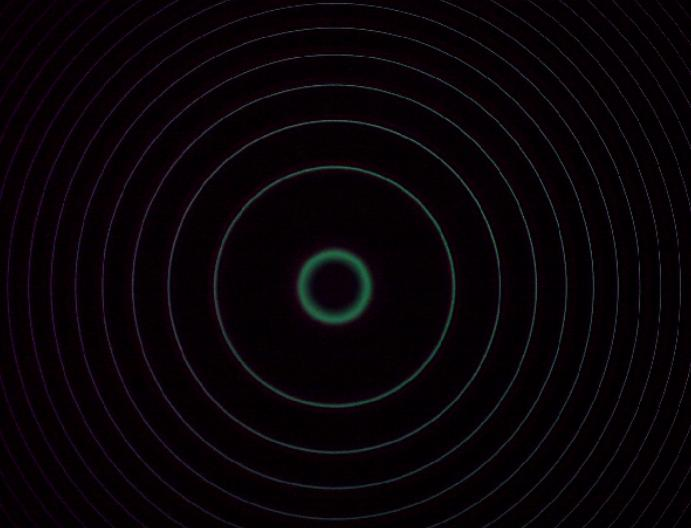
\includegraphics[width=0.5\textwidth]{Images/B=0Pattern}
		\caption{Interference pattern of the 546.1nm mercury line with no applied magnetic field. The interference lines are singular.}
		\label{fig:B=0Pattern}
	\end{figure}
 
	 \begin{table}[h]
	 	\centering
	 	\begin{tabular}{l|l}
	 		k & Radius (m) \\ \hline
	 		4 & 0.7956 $\pm$ $0.1\times10^{-3}$    \\
	 		3 & 0.6911 $\pm$ $0.2\times10^{-3}$    \\
	 		2 & 0.5678 $\pm$ $0.1\times10^{-3}$    \\
	 		1 & 0.4096 $\pm$ $0.1\times10^{-3}$   
	 	\end{tabular}
	 	\caption{\textbf{Interference ring radii of the mercury 546.1 nm spectra with no magnetic field.}}
	 	\label{tab:B0Data}
	 	
	 \end{table}
	\subsection{Spectra Through a Perpendicular Magnetic Field}
		The first observations were made such that the mercury lamp was viewed through a magnetic field perpendicular to the travel of the mercury spectra, as is shown in \ref{subfig:PerpFieldConfig}.
		With this magnetic field configuration, observations were made with the polarizer at $0\degree$ (Parallel to the field lines), and $90\degree$ (perpendicular to the field lines).
		This allowed us to observe the hyperfine spectral lines with polarization parallel and perpendicular to the magnetic field lines, which correspond to photons created in $\Delta M_z = 0$ and $\Delta M_Z = \pm1$ transitions, respectively, of the mercury electrons.
		\subsubsection{Spectra with Field-Perpendicular Polarization}
			
			With the polarizer set to $90\degree$, we observed the mercury spectra with polarization perpendicular to the applied magnetic field. A distinct triple ring structure can be seen Figure \ref{fig:Triplet90deg} in which each interference ring consists of a bright central ring surrounded by two fainter rings. 
			
			\begin{figure}
				\centering
				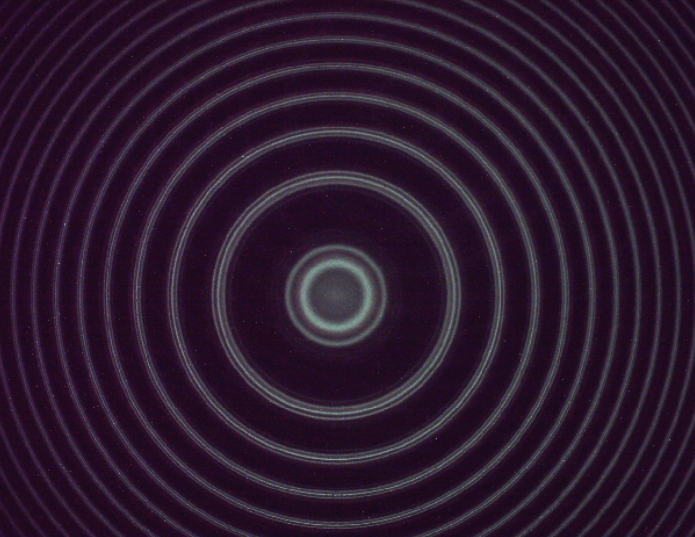
\includegraphics[width=0.5\textwidth]{Images/Run1_ParallelPolarizer}
				\caption{Interference pattern of the mercury spectrum with a ~1T applied magnetic through a polarizer oriented perpendicular to the magnetic field lines. The interference rings correspond to light produced by $\Delta M_z = 0$ transitions polarized perpendicularly to the magnetic field.}
				\label{fig:Triplet90deg}
			\end{figure}
			
			Using PASCO Software, The radii of the inner and outer rings of the $k=1$ through $k=4$ interference rings were measured.
			These radii are given in Table \ref{tab:RadiusMeasurements}.
			
			\begin{table*}[]
				\centering
				\begin{tabular}{l|lll}
					k = 1 & & & \\
					Measurements & $R+$ (m) & $R-$ (m)  & $\Delta$R (m) \\ \hline
					1         & 0.4282 & 0.3893  & 0.0389 \\
					2         & 0.4278 & 0.3896  & 0.0382 \\
					3         & 0.4275 & 0.3887  & 0.0388 \\
					Mean      & $0.4278\pm0.4\times10^{-3}$       & $0.3892\pm0.5\times10^{-3}$        & $0.039\pm0.4\times10^{-3}$ \\ \hline
					k = 2 & & & \\
					Measurements & $R+$ (m) & $R-$ (m)  & $\Delta$R (m) \\ \hline
					1           & 0.5819 & 0.5539 & 0.0280 \\
					2           & 0.5815 & 0.5536 & 0.0279 \\
					3           & 0.5818 & 0.5536 & 0.0282 \\
					Mean        & $0.5817\pm0.2\times10^{-3}$ & $0.5537\pm0.2\times10^{-3}$ & $0.0280\pm0.2\times10^{-3}$ \\ \hline
					k = 3 & & & \\
					Measurements & $R+$ (m) & $R-$ (m)  & $\Delta$R (m) \\ \hline
					1    & 0.7035 & 0.679  & 0.0245 \\
					2    & 0.7033 & 0.6798 & 0.0235 \\
					3    & 0.7025 & 0.6805 & 0.0220 \\
					Mean & $0.7031\pm0.5\times10^{-3}$ & $0.6798\pm0.8\times10^{-3}$ & $0.0233\pm0.001$ \\ \hline
					k = 4 & & & \\
					Measurements & $R+$ (m) & $R-$ (m)  & $\Delta$R (m) \\ \hline
					1    & 0.8058 & 0.7861 & 0.02  \\
					2    & 0.8057 & 0.7865 & 0.02  \\
					3    & 0.8059 & 0.7857 & 0.02  \\
					Mean & $0.8058\pm0.1\times10^{-3}$ & $0.7861\pm0.4\times10^{-3}$ & $0.020\pm0.001$
				\end{tabular}
				
				
				\caption{\textbf{Radius measurements of the hyperfine structure of the k=1 through k=4 interference rings with a 1T magnetic field and $\mathbf{90\degree}$ polarization.}}
				\label{tab:RadiusMeasurements}
			\end{table*}
			
		\subsubsection{Spectra with Field-Parallel Polarization}
		\begin{figure}
			\centering
			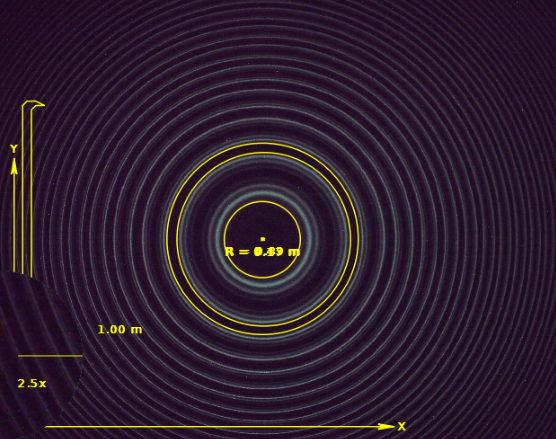
\includegraphics[width=0.5\textwidth]{Images/Run2_PerpendicularPolarizer}
			\caption{Interference pattern in the presence of an external magnetic field with a polarizer oriented parallel to the magnetic field lines.}
			\label{fig:Run2_0Deg}
		\end{figure}

		
	\subsection{Spectra Along an Axial Magnetic Field}
	
	\subsection{Measurement of the Bohr Magneton} \label{subsec:BohrMagneton}
		With the precise measurement of spectral line splitting in the presence of the perpendicular magnetic field, it was possible to measure the value of the Bohr magneton.
		
		\begin{table}[]
			\centering
			\begin{tabular}{l|l}
				$\mathbf{k}$    & $\mathbf{\mu_B \ (J/T)}$ \\ \hline
				\textbf{1}    & $9.16\times10^{-24}$   \\
				\textbf{2}    & $9.24\times10^{-24}$   \\
				\textbf{3}    & $9.36\times10^{-24}$   \\
				\textbf{4}    & $9.10\times10^{-24}$   \\ \hline
				\textbf{Mean} & $9.22\times10^{-24}\pm0.6\times10^{-24}$  
			\end{tabular}
			\caption{\textbf{Calculated values of the Bohr magneton $\mathbf{\mu_B}$ for each interference ring, and the mean calculated value for all interference rings.}}
			\label{tab:BohrCalcs}
		\end{table}
	

\section{Conclusion} \label{sec:Conclusion}

\bibliographystyle{ieeetr}
\bibliography{ZeemanPaper}

\end{document}
